\documentclass[a4paper, 10pt, conference]{ieeeconf}

% Framework thanks to Vu Dinh Quang Dat
\usepackage{relsize}
\usepackage{sectsty}
\usepackage{amsmath}
\usepackage{amssymb}
\usepackage[utf8]{inputenc}
\usepackage[english]{babel}
\usepackage{titlesec}
\usepackage{graphicx} 
\usepackage{wrapfig}
\usepackage{blindtext}
\usepackage{hyperref}
\usepackage{indentfirst}

\title{\LARGE \bf
	Modelling Crimes using Gaussian Processes\\
	\normalsize CS4246 Project: Planning and Decision Making in the Real World
}

\author{
	\bf \small CS4246 Team 05 Members:\\
	\small Choo Boon Yong Martin, A0132760M\\
	\small Leow Yijin, A0131891E\\
	\small Tan Soon Jin, A0112213E\\
	\small Teo Qi Xuan, A0124206W\\
	\small Won Jun Ru Daphne, A0126172M\\
	\small Zhu Liang, A0093910H\\
}


\begin{document}		
	
	\pdfinfo{
		/Title Modelling Crimes using Gaussian Processes
		/Author Martin, Yijin, Soon Jin, Qi Xuan, Daphne, Zhu Liang
	}
	
	\maketitle
	\thispagestyle{empty}
	\pagestyle{empty}
	
	
	%%%%%%%%%%%%%%%%%%%%%%%%%%%%%%%%%%%%%%%%%%%%%%%%%%%%%%%%%%%%%%%%%%%%%%%%%%%%%%%%
	
	\begin{abstract}
	\begin{quote}
		Efficient allocation of police resources is needed to better combat crime. Although both heatmaps (kernel-based intensity smoothing) and Gaussian Processes (GP) have been explored as a way of modelling crime, they have never been used in tandem. 
		In this paper. we propose an innovative way of modelling crime density combined with  demographics to produce a heatmap of risk assessment of crime in a area. This will form an objective guide for law enforcers and planners to better allocate manpower and offer help to the communities.
	\end{quote}
	\end{abstract}
	
	%%%%%%%%%%%%%%%%%%%%%%%%%%%%%%%%%%%%%%%%%%%%%%%%%%%%%%%%%%%%%%%%%%%%%%%%%%%%%%%%
	
	%%%%%%%%%% Section 1
	\section{Introduction}
	
	In this paper, we propose the use of the Gaussian Process (GP) to model the spread of crimes in the District of Columbia (DC).
	The paper will discuss the important requirements of crime models and how we exploit the desirable properties of GP models and the qualitative advantages GP models provide to address the requirements.\\ \\

	The paper will also explain how our GP model fits and predicts the crime data, additional insights gained as well as novel modifications of the GP to enhance it. 
	Notably, we touch upon how we visualize the output to provide a novel and unprecedented way of interpreting GPs and how how the DC authorities can interpret the output.\\ \\

	We then discuss the experimental evaluation of our GP model, particularly how we test it and how the model performs in comparison with other regression models. 
	
	%%%%%%%%%%%%%%%%%% Section 2
	\section{Gaussian Process and Crime}

	In this section, we will briefly describe GPs and our GP model. We then highlight the important requirements of crime modelling, and how our proposed application exploits the desirable properties of GP and its qualitative advantages, as well as how our GP model fits the requirements of crime modelling exactly. 
	Finally, we show a sample output of our model and discuss how the relevant authorities can interpret and exploit the output of the GP model and interact with it.\\ \\

	\subsection{Gaussian Process}
	
	A Gaussian process is a collection of random variables, any finite number of which have a joint Gaussian distribution.
	GP is a non-parametric technique to generalize a set of random variables (r.v.) as a distribution over functions with an infinite dimension. \cite{c01}
	It is defined by its mean and variance. We define x as a random input variable, $\mu (x)$ as its mean function and $\kappa$ (x, x') as its covariance function resulting in \[f(x) \sim GP(\mu (x), \kappa (x, x')) \]
	Realistically, a GP model is affected by noise, as expressed $y_i = f(x_i) + \epsilon_i$ where $\epsilon_i \sim N(0, \sigma^2_n)$.
	Given observation $\mathbf{y} = [y_1, y_2, \ldots, y_n]^T$, GP will try to infer  $ p(f(\text{x*} | \textbf{y}) \triangleq \mathcal{N}(f(\text{x*}); \mu, \sigma^2)$ where $\mu$ is the prediction and $\sigma^2$ is the predictive variance. 
	
	\subsection{Our Model}
	
	In our GP model, we model all the crimes in a particular district to predict the time and an approximate area at which future crimes are likely occur.
	We first input various features of past crimes such the Police Service Area (PSA) in charge of the area and the time the crime occurred.
	After processing, we output a heatmap of the likelihood of a specific type of crime occurring in specific areas at specific times, an original and groundbreaking way of visualizing output of GPs.
	
	\subsection{Important Requirements of Crime Models}
	
	Crime occurs continuously and randomly. It is possible for days to go by without any incidents reported, and also possible for multiple incidents to be reported in the same hour.
	Another important factor is that it is possible for a crime to go either undetected or unreported. Thus the model will need to be able to accurately model data with uneven occurrence rates.
	Furthermore, crime can occur as a result of a large number of interdependent factors, most of them unknown and situation dependent. What drives one criminal to commit crimes may not be the same for another.
	Therefore, the model should not make any assumptions on the features. We should also be able to update the model as more crime occurs, allowing an up-to-date model.\\ \\
	\blindtext
	
	\subsection{Desirable Properties of Gaussian Processes}
	
	We thus choose to use GP models to exploit the many advantages it provides in the context of crime.
	The non-parametric nature of GP allows us to model the crime data without making assumptions on the features of crimes.
	The Bayesian property also allows us to update our GP model with information about new crimes as they continue to happen, letting us capture more information captured about the data as crimes occur.\\ \\

	On the contrary, using a parametric model such as linear regression lacks flexibility to adjust with new datasets, and also requires us to assume features of the crime data.
	It would also be harder to update with new information.\\ \\

	The uneven occurrence rate of crimes creates an uneven sampling rate of sorts.
	Even then, the GP model allows us to use all of the information in the crime dataset to model and predict future crimes.

	The ‘Broken Window’ theory suggests that an area where a crime has occurred is likely to have more crime. \cite{c07}
	Following this theory, it is highly likely that the crime occurrences in a particular neighbourhood are highly correlated with one another.
	GP model thus provides a good fit for the data.

	\subsection{Output and Interpretation}
	A further advantage of the GP model is that through the predictive mean and uncertainty, we obtain a probability of the crime occurring at a certain area and at a certain time.
	This probability is essential for generating our new and innovative heatmap which will allow the relevant authorities to deploy resources accordingly.
	This is something that regression models such as linear and polynomial regression cannot provide.\\ \\

	Our model outputs a relative risk heatmap for each type of crime, calculated with respect to expected number of crimes, based on the population in a PSA.
	The heatmap is intuitive to interpret, with darker areas being riskier areas.
	It is also possible to output heatmaps of individual crimes if the authorities choose to do so.

	\begin{figure}[!ht]
		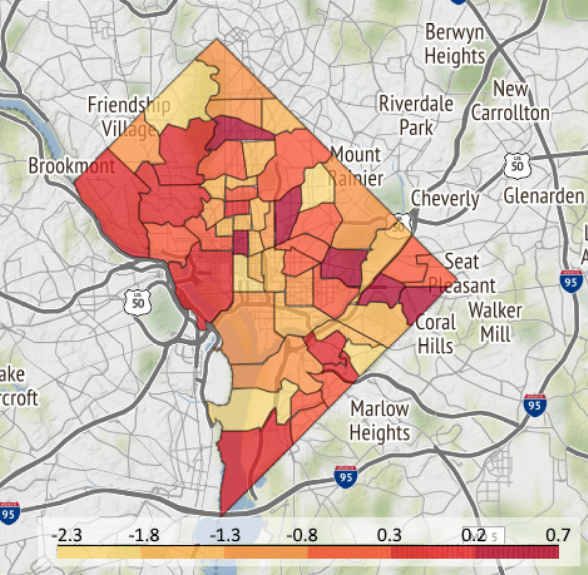
\includegraphics[width=\linewidth]{./p1.png}
		\caption{June 2016 Week 1 Predicted Burglary Log Relative Risk.}
		\label{p1}
	\end{figure}

	The intuitive and innovative heatmap output can be advantageous in many ways.
	As we output a heatmap for each type of crime, police officers are able to do pre-emptive tactical planning, based on both the risk level and the types of crimes expected to occur.
	The public can also be informed of the risk of going to those areas. 
	Finally, detecting anomalies from the predicted amount can signal something greater happening, such as gang formation.
	
	%%%%%%%%%%%%%% Section 3
	\section{Technical Approach}
	
	In this section, we will discuss the modelling approach taken for our model, some additional insights gained from this modelling and why our heatmap is really cool.
	
	\subsection{Modelling Approach}
	Using the DC Crime Map dataset, we split the input by PSA and by week, and train the model on specific crime counts such as robbery, assault and burglary for the period of March to May 2016. 
	As we are dealing with count data that we cannot assume to be mutually independent, unlike the Poisson Process, we model a latent relative risk surface that generates the Cox process (inhomogeneous Poisson Process).
	This is similar to Log Gaussian Cox Process (LGCP) used to model point process.
	To predict the likelihood of a crime, we use a poisson distribution. Due to its non-Gaussian characteristic, we approximate an inference with Laplace Approximation by utilizing the second order Taylor series, or the following formula:
	\[p(y|f) = \prod_{s,t}Poisson(y_{s,t}|exp(f(s,t))\cdot e_s)\]

	In selecting the kernel, we combine multiple kernels to investigate the effect of different input dimensions:
	\[K((s,t),(s',t')) = k_s(s,s')+k_t(t,t')+k_{st}((s,t),(s',t'))\]

	We use the Matern 3/2 kernel for space and Radial Basis Function kernel for time.
	Unlike Flaxman (2016), we choose to ignore the periodic kernel as we only deal with 3 months training data for now, which does not show any periodicity.
	We then maximize the marginal likelihood by optimizing using Limited-Memory Broyden–Fletcher–Goldfarb–Shanno (LBFGS).
	We chose the LBFGS method as it gave the best result of all the methods tried, including Scaled Conjugate Gradients and Truncated Newton method.
	
	\subsection{Additional Insight}
	Through the undertaking of this project, we have derived several additional insights about the GP model:
	\begin{enumerate}
		\item {\bf Pattern Discovery:} We can use a more expressive kernel from a learned covariance function to learn hidden representations of data. \cite{c03}
		\item {\bf Feature Selection:} It is possible to use ARD (Automatic Relevance Determination) covariance function to perform feature selection on different inputs for a crime problem. \cite{c03}
		\item {\bf Log-Cox Gaussian Process:} It is possible to apply LGCP to investigate the contagious effect of crime. \cite{c05}
		\item {\bf Multiple Output GP:} We applied multiple task learning, that is, information shared between the tasks to compensate for missing data.
		\item {\bf Stationarity of data:} We experimented with non-stationary kernel, assuming the data was stationary.
		\item {\bf Mean Function:} We learned the Importance of setting mean function properly to indicate bias.
		\item {\bf Incorporation of Side Data:} Another advantage of the GP is the possibility of incorporating side information by coupling together multiple Probabilistic Matrix Factorization problems. \cite{c02}
	\end{enumerate}
	
	\subsection{Novel and Interesting Heatmap}
	Although both GP and heatmaps (kernel-based intensity smoothing) have already been used in crime prediction separately, there has been no recorded instances of GP models that can produce a visually interpretable heatmap or output.\\ \\
	As discussed in the earlier Interpreting Outputs section, our group has thus focused on the visualization of the GP model output in order to exploit both the many advantages of GP and the intrinsic user-friendliness of heatmaps.
	In doing so, we have created a novel heatmap GP visualization that will enable the relevant authorities will be able to better make an informed decision on how to best allocate police resources.
	
	%%%%%%%%%%%%%%%% Section 4
	\section{Experimental Evaluation}
	The usefulness of a GP model depends on many factors. As such, there is a need to empirically evaluate its performance.
	In particular, we focus on how our model will be used to enable efficient allocation of police resources to combat crime.

	\subsection{Testing of GP}
	For efficient allocation of police resources to combat crime, we place an emphasis on accuracy of crime predicted and ease of interpreting output.
	As we do not know of any other models that output a visual heatmap, we thus focus our tests on accuracy.
	To measure accuracy, we use root mean square error (RMSE) to benchmark our model against the state-of-the-art alternatives \cite{c06}
	

	\begin{table}[!ht]
		\resizebox{\linewidth}{!} {
		\begin{tabular}{| l | l | l | }
		\hline
		& Our Model & State-of-the-Art Model \\ \hline
		In-Sample Error & 1.140 & 4.829\\
		\hline
		\end{tabular}
		}
		\caption{RMSE of our Model against state-of-the-art models.}
		\label{t1}
	\end{table}
	
	We can see that our model is better than state-of-the-art-models in predicting in-sample errors.

	\subsection{Comparison with Current Methods}
	
	To get an indication of how useful our model is, we then perform the same test on out-of-sample data.
	We do not know how the DC authorities currently allocates police resources, however we believe it would be reasonable to assume that they would patrol areas with high crime rates previously, i.e. a naive model.
	We thus compare our model against both the state of the art model and a naive forecast model with Holt-Winters smoothing.
	
	\begin{figure}[!ht]
		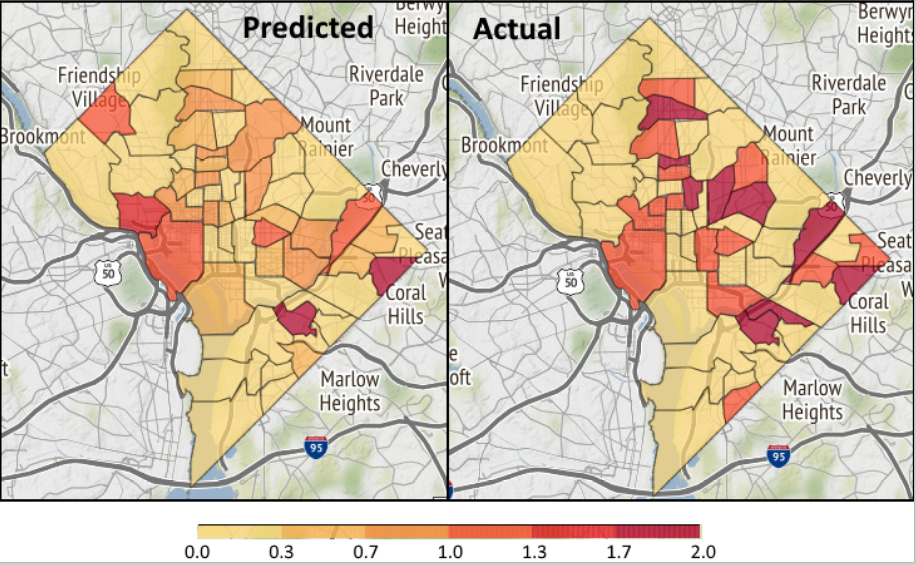
\includegraphics[width=\linewidth]{./p2.png}
		\caption{Predicted and Actual Robbery Crimes in June 2016 Week 1.}
		\label{p2}
	\end{figure}

	\begin{table}[!ht]
		\begin{tabular}{| p{1cm} | l | p{2cm} | p{1.5cm} | }
		\hline
		& Our Model & State-of-the-Art Model & Holt-Winters \\ \hline
		Out-Sample Error & 6.325 & 5.080 & 6.855\\
		\hline
		\end{tabular}
		\caption{RMSE of our model against state-of-the-art models and naive with Holt-Winters.}
		\label{t2}
	\end{table}

	As can be observed, although our model underperforms when compared to the state-of-the-art model, it outperforms the Holt-Winters method.
	However, we believe the  tradeoff in accuracy is compensated by the ease of interpreting the output, which allows for better allocation of police resources.
	
	%%%%%%%%%% Section 5
	\section{Conclusion}
	In this paper, we have proposed an innovative way of combining the rich class of Gaussian Processes and the visually interpretable heatmap to create an easily interpretable risk assessment of crime in a area.
	Although our model slightly underperforms when compared with the latest state-of-the-art model, we believe that the slight dip in accuracy is an acceptable trade-off for the more user-friendly output.
	It is also likely that enhancing our model with side information that the authorities have access to will enable us to outperform the state-of-the-art model.
	
	%%%%%%%%% Section 6
	\section{Members}
	\begin{itemize}
		\item {\bf Choo Boon Yong Martin (A0132760M), Leow Yijin (A0131891E) and Tan Soon Jin (A0112213E)} were in charge of modelling the data.
		\item {\bf Teo Qi Xuan (A0124206W) and Won Jun Ru Daphne (A0126172M)} were in charge of writing the report.
		\item {\bf Zhu Liang (A0093910H)} was in charge of processing the data and visualization.
	\end{itemize}

	%%%%%%%%%% Section 7
	\begin{thebibliography}{9}
	\bibitem{c01}
	McDubb, D. (2010).
	\textit{Gaussian Processes.}
	Lecture, Massachusetts Institute of Technology
	
	\bibitem{c02}
	Ryan Prescott Adams, George E. Dahl \& Iain Murray (2014).
	\textit{Incorporating Side Information in Probabilistic Matrix Factorization with Gaussian Processes.}
	Twenty-Sixth Conference on Uncertainty in Artificial Intelligence (UAI2010). arXiv:1408.2039

	\bibitem{c03} 
	Wilson, A.G., Adams, R.P. (2010).
	\textit{Gaussian Process Kernels for Pattern Discovery and Extrapolation.}
	The 30th International Conference on Machine Learning. JMLR W\&CP 28 (3) :1067-1075, 2013
	
	\bibitem{c04} 
	Ghahramani, Z. (2010).
	\textit{A Tutorial on Gaussian Processes.}
	Lecture, University of Cambridge
	
	\bibitem{c05}
	Clifton, D. (2016).
	Log Gaussian Cox Processes. Presentation, Computational Health Informatics Group Meeting.

	\bibitem{c06}
	Flaxman, S. (2016).
	A General Approach to Prediction and Forecasting Crime Rates with Gaussian Processes. Retrieved October 13, 2016, from https://www.ml.cmu.edu/research/dap-papers/dap\_flaxman.pdf

	\bibitem{c07}
	Wilson, J. Q., \& Kelling, G. (n.d.).
	Broken Window Theory | Missoula, MT - Official Website. Retrieved October 13, 2016, from http://www.ci.missoula.mt.us/881/Broken-Window-Theory

	
	\end{thebibliography}
\end{document}